%===========================================================
% 04_binarization.tex - 图像二值化
%===========================================================

\section{图像二值化}

%-----------------------------------------------------------
% Frame 1: 什么是二值化
%-----------------------------------------------------------
\begin{frame}{什么是二值化？}
    \begin{columns}
        \column{0.5\textwidth}
        \begin{block}{定义}
            \begin{itemize}
                \item 将灰度图像转换为只有\textbf{黑白}两种颜色
                \item 像素值：0（黑）或 255（白）
                \item 公式：$B(x,y) = \begin{cases} 0 & I(x,y) < T \\ 255 & I(x,y) \geq T \end{cases}$
            \end{itemize}
        \end{block}

        \column{0.5\textwidth}
        \begin{alertblock}{为什么重要？}
            \begin{itemize}
                \item 简化图像，便于分析
                \item \highlight{OCR 识别前必经步骤}
                \item 边缘检测基础
                \item 文档扫描核心
            \end{itemize}
        \end{alertblock}
    \end{columns}

    \begin{center}
        \begin{tikzpicture}[scale=0.8]
            \node[rectangle, draw, minimum width=3cm, minimum height=2cm] (gray) at (0,0) {灰度图};
            \node[rectangle, draw, minimum width=3cm, minimum height=2cm, fill=black!20] (thresh) at (5,0) {阈值 $T$};
            \node[rectangle, draw, minimum width=3cm, minimum height=2cm] (bin) at (10,0) {二值图};

            \draw[->, thick] (gray) -- (thresh);
            \draw[->, thick] (thresh) -- (bin);
        \end{tikzpicture}
    \end{center}
\end{frame}

%-----------------------------------------------------------
% Frame 2: 二值化应用场景
%-----------------------------------------------------------
\begin{frame}{二值化应用场景}
    \begin{columns}
        \column{0.5\textwidth}
        \begin{block}{典型应用}
            \begin{enumerate}
                \item \highlight{OCR 文字识别}：将文字与背景分离
                \item 文档扫描：去除彩色背景
                \item 边缘检测：提取轮廓
                \item 血细胞计数：分离细胞
                \item 车牌识别：定位车牌
            \end{enumerate}
        \end{block}

        \column{0.5\textwidth}
        \begin{figure}
            \centering
            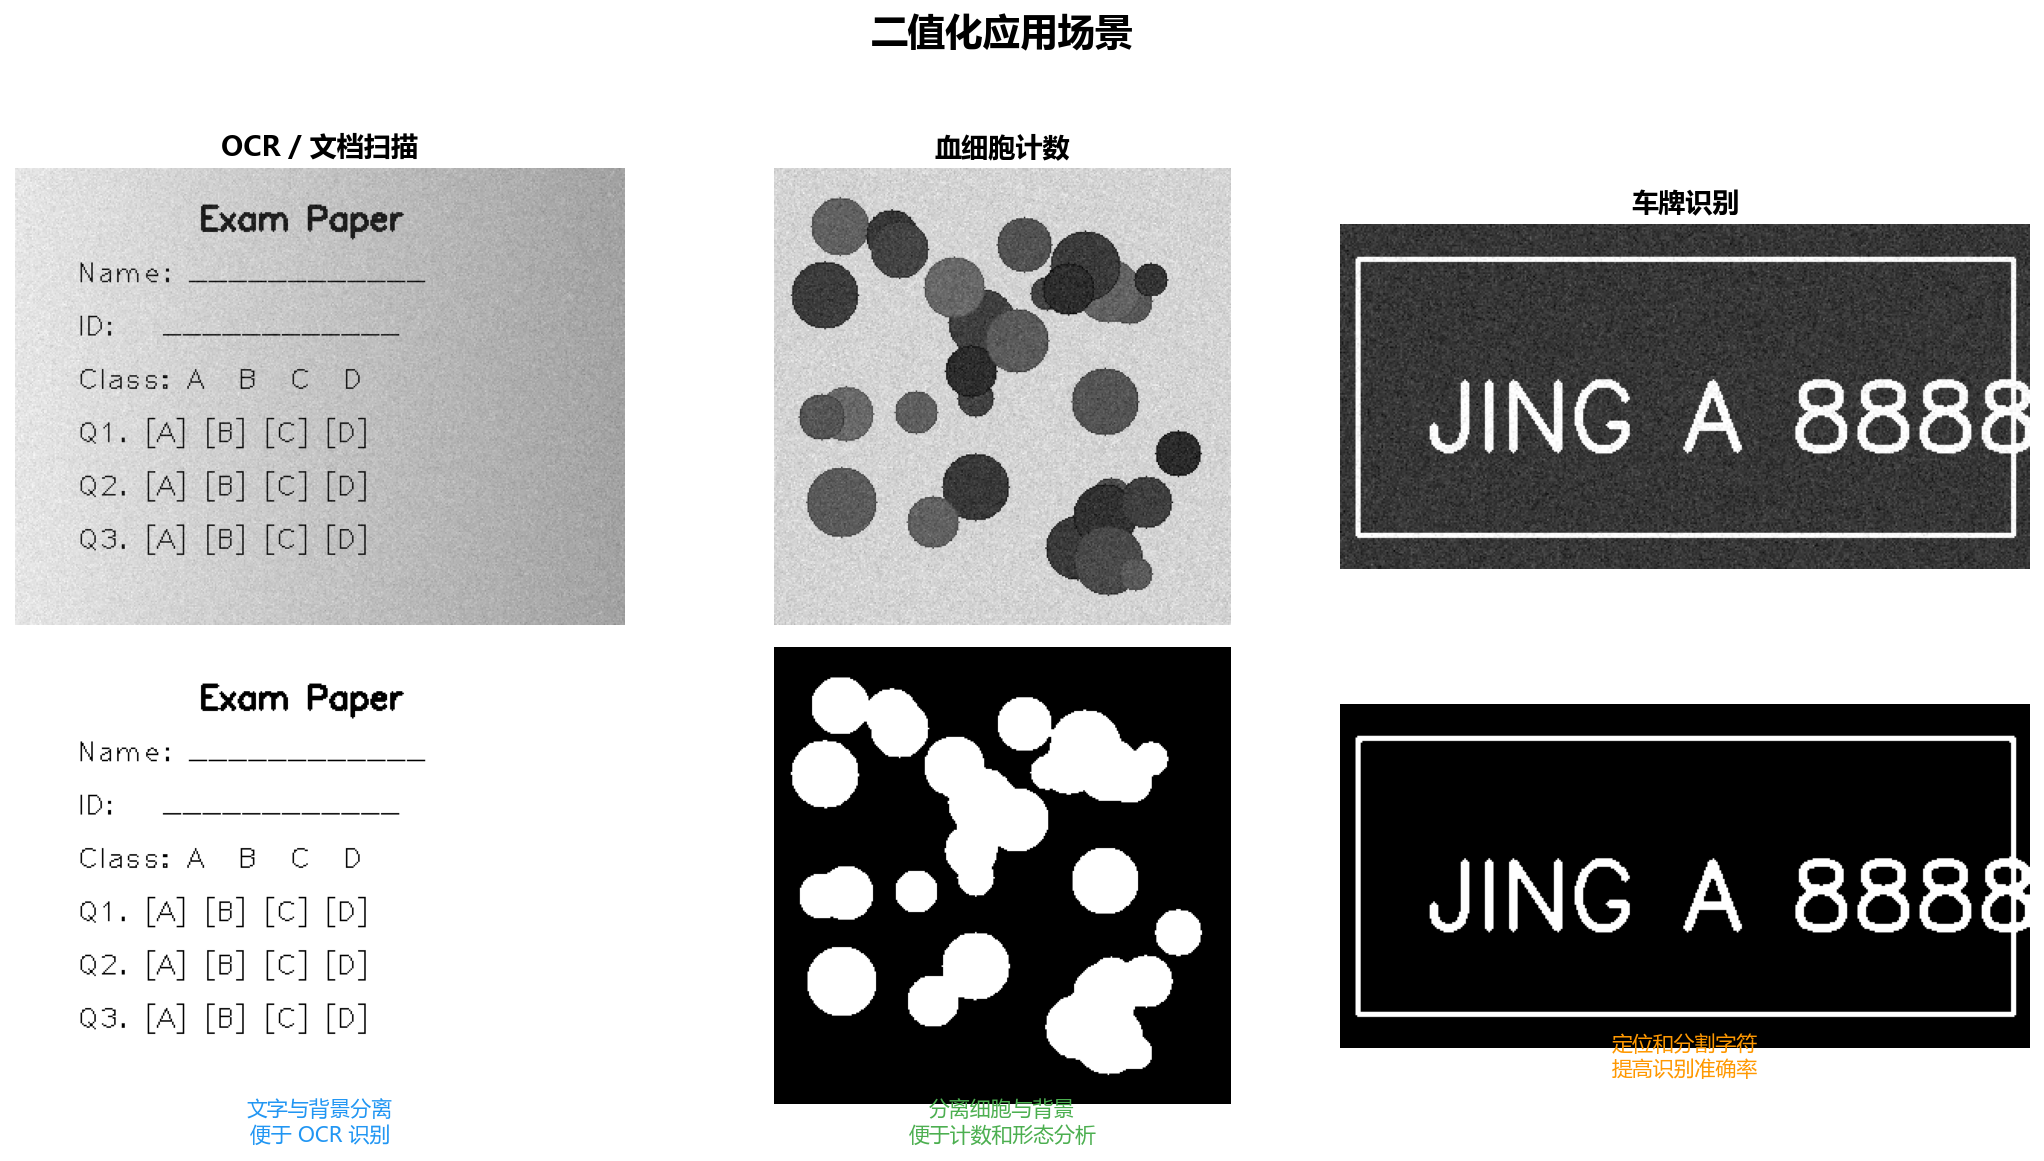
\includegraphics[width=\textwidth]{images/binarization_applications.png}
            \caption{三种典型场景的二值化效果}
        \end{figure}
    \end{columns}
\end{frame}

%-----------------------------------------------------------
% Frame 3: 全局阈值法
%-----------------------------------------------------------
\begin{frame}[fragile]{全局阈值法}
    \textbf{原理：} 使用固定阈值 $T$ 进行分割

    \begin{columns}
        \column{0.5\textwidth}
        \begin{lstlisting}[basicstyle=\ttfamily\scriptsize]
import cv2
import numpy as np

# 读取灰度图
gray = cv2.imread('exam.jpg', 0)

# 方法1: 固定阈值 127
_, binary1 = cv2.threshold(
    gray, 127, 255, cv2.THRESH_BINARY
)

# 方法2: 反转二值化
_, binary2 = cv2.threshold(
    gray, 127, 255, cv2.THRESH_BINARY_INV
)

# 方法3: 截断
_, binary3 = cv2.threshold(
    gray, 127, 255, cv2.THRESH_TRUNC
)

# 方法4: 零化
_, binary4 = cv2.threshold(
    gray, 127, 255, cv2.THRESH_TOZERO
)
        \end{lstlisting}

        \column{0.5\textwidth}
        \begin{block}{阈值类型}
            \begin{itemize}
                \item \code{THRESH\_BINARY}: 大于 T 设为 255
                \item \code{THRESH\_BINARY\_INV}: 反转
                \item \code{THRESH\_TRUNC}: 截断到 T
                \item \code{THRESH\_TOZERO}: 小于 T 设为 0
            \end{itemize}
        \end{block}

        \begin{alertblock}{问题}
            固定阈值需要手动尝试，不适合光照不均图像
        \end{alertblock}
    \end{columns}
\end{frame}

%-----------------------------------------------------------
% Frame 4: Otsu 自适应阈值
%-----------------------------------------------------------
\begin{frame}[fragile]{Otsu 自适应阈值}
    \textbf{原理：} 自动寻找最佳阈值（直方图双峰时效果好）

    \begin{columns}
        \column{0.5\textwidth}
        \begin{block}{算法思想}
            \begin{enumerate}
                \item 假设直方图呈双峰分布
                \item 寻找两峰之间的谷底作为阈值
                \item 最大化类间方差 (Otsu 方法)
            \end{enumerate}
        \end{block}

        \column{0.5\textwidth}
        \begin{lstlisting}[basicstyle=\ttfamily\scriptsize]
import cv2
import numpy as np

gray = cv2.imread('document.jpg', 0)

# Otsu 方法自动找阈值
_, otsu = cv2.threshold(
    gray,           # 原图
    0,              # 阈值（设为0，Otsu自动计算）
    255,            # 最大值
    cv2.THRESH_BINARY + cv2.THRESH_OTSU
)

# 对比效果
fig, axes = plt.subplots(1, 3, figsize=(12, 4))
axes[0].imshow(gray, cmap='gray')
axes[0].set_title('原图')

axes[1].imshow(cv2.threshold(gray, 127, 255, cv2.THRESH_BINARY)[1], cmap='gray')
axes[1].set_title('固定阈值127')

axes[2].imshow(otsu, cmap='gray')
axes[2].set_title('Otsu自适应')
plt.show()
        \end{lstlisting}
    \end{columns}

    \begin{alertblock}{适用场景}
        背景和前景灰度差异明显（如文档、书页）
    \end{alertblock}
\end{frame}

%-----------------------------------------------------------
% Frame 5: 自适应阈值
%-----------------------------------------------------------
\begin{frame}[fragile]{自适应阈值}
    \textbf{原理：} 根据邻域计算局部阈值

    \begin{columns}
        \column{0.5\textwidth}
        \begin{block}{两种方法}
            \begin{itemize}
                \item \code{ADAPTIVE\_THRESH\_MEAN}: 邻域均值
                \item \code{ADAPTIVE\_THRESH\_GAUSSIAN}: 高斯加权
            \end{itemize}
        \end{block}

        \begin{block}{参数}
            \begin{itemize}
                \item \code{blockSize}: 邻域大小（奇数）
                \item \code{C}: 从均值中减去的常数
            \end{itemize}
        \end{block}

        \column{0.5\textwidth}
        \begin{lstlisting}[basicstyle=\ttfamily\scriptsize]
import cv2

gray = cv2.imread('exam.jpg', 0)

# 方法1: 基于均值
adaptive_mean = cv2.adaptiveThreshold(
    gray, 255,
    cv2.ADAPTIVE_THRESH_MEAN_C,
    cv2.THRESH_BINARY,
    blockSize=11,
    C=2
)

# 方法2: 基于高斯（更常用）
adaptive_gaussian = cv2.adaptiveThreshold(
    gray, 255,
    cv2.ADAPTIVE_THRESH_GAUSSIAN_C,
    cv2.THRESH_BINARY,
    blockSize=11,
    C=2
)

# 参数调优建议
# - blockSize 越大，平滑效果越强
# - C 越大，二值化越严格
        \end{lstlisting}
    \end{columns}

    \begin{alertblock}{GUI演示程序：\code{gui\_03\_binarization.py}}
		运行 \code{python gui\_launcher.py} 选择“二值化演示”，可交互调节阈值方法、块大小和C值
    \end{alertblock}
\end{frame}

%-----------------------------------------------------------
% Frame 6: 三种方法对比表
%-----------------------------------------------------------
\begin{frame}{二值化方法对比}
    \begin{table}
        \centering
        \begin{tabular}{p{2.5cm}p{3cm}p{4cm}p{2cm}}
            \toprule
            \textbf{方法} & \textbf{原理} & \textbf{适用场景} & \textbf{缺点} \\
            \midrule
            全局固定阈值 & 固定值 $T=127$ & 背景均匀 & 不抗光照变化 \\
            Otsu & 最大化类间方差 & 文档、书页 & 对噪声敏感 \\
            自适应 & 局部邻域计算 & 光照不均 & 可能有块效应 \\
            \bottomrule
        \end{tabular}
    \end{table}

    \begin{alertblock}{实战建议}
        \begin{itemize}
            \item 文档扫描：Otsu 或自适应阈值
            \item 试卷答题卡：自适应阈值 + 后处理
            \item \highlight{组合使用：中值滤波去噪 + 自适应阈值}
        \end{itemize}
    \end{alertblock}
\end{frame}

%-----------------------------------------------------------
% Frame 7: 代码实战 - 二值化函数
%-----------------------------------------------------------
\begin{frame}[fragile]{代码实战：二值化函数}
    \begin{lstlisting}[basicstyle=\ttfamily\scriptsize]
import cv2
import numpy as np

def binarize_image(image_path, method='otsu', blockSize=11, C=2):
    """
    二值化函数

    Args:
        image_path: 图像路径
        method: 'otsu', 'adaptive_mean', 'adaptive_gaussian'
        blockSize: 自适应阈值块大小
        C: 阈值偏移量

    Returns:
        二值化图像
    """
    # 读取灰度图
    gray = cv2.imread(image_path, 0)
    if gray is None:
        raise ValueError(f"无法读取图像: {image_path}")

    # 根据方法选择
    if method == 'otsu':
        _, binary = cv2.threshold(
            gray, 0, 255,
            cv2.THRESH_BINARY + cv2.THRESH_OTSU
        )
    elif method == 'adaptive_mean':
        binary = cv2.adaptiveThreshold(
            gray, 255,
            cv2.ADAPTIVE_THRESH_MEAN_C,
            cv2.THRESH_BINARY,
            blockSize, C
        )
    elif method == 'adaptive_gaussian':
        binary = cv2.adaptiveThreshold(
            gray, 255,
            cv2.ADAPTIVE_THRESH_GAUSSIAN_C,
            cv2.THRESH_BINARY,
            blockSize, C
        )
    else:
        raise ValueError(f"未知方法: {method}")

    return binary

# 测试
if __name__ == '__main__':
    result = binarize_image('document.jpg', method='adaptive_gaussian')
    cv2.imshow('Result', result)
    cv2.waitKey(0)
    \end{lstlisting}

    \begin{alertblock}{挑战任务}
        添加后处理步骤：形态学操作去除噪点
    \end{alertblock}
\end{frame}

%-----------------------------------------------------------
% Frame 8: 代码找茬
%-----------------------------------------------------------
\begin{frame}[fragile]{代码找茬：找出 BUG}
    \begin{block}{问题：下面的代码有什么问题？}
        \begin{lstlisting}[basicstyle=\ttfamily\scriptsize]
import cv2
import numpy as np

def buggy_binarize(img):
    """有BUG的二值化函数"""

    # BUG 1: 忘记转灰度
    result = cv2.threshold(img, 127, 255, cv2.THRESH_BINARY)
    return result  # 返回的是tuple，不是图像！

def correct_binarize(img):
    """正确的写法"""
    # 确保是灰度图
    if len(img.shape) == 3:
        gray = cv2.cvtColor(img, cv2.COLOR_BGR2GRAY)
    else:
        gray = img

    # 正确处理返回值
    _, result = cv2.threshold(gray, 127, 255, cv2.THRESH_BINARY)
    return result

# 测试
img = cv2.imread('test.jpg')
cv2.imshow('Result', correct_binarize(img))  # 修复后
cv2.waitKey(0)
        \end{lstlisting}
    \end{block}

    \begin{alertblock}{找茬提示}
        \begin{itemize}
            \item BUG 1: \code{cv2.threshold} 返回两个值
            \item BUG 2: 彩色图直接二值化会出错
        \end{itemize}
    \end{alertblock}
\end{frame}
